\documentclass{report}
\usepackage[utf8]{inputenc}
\usepackage{fixlatvian}
\usepackage{verbatim}
\usepackage{graphicx}
\usepackage{pgfplots}


\usepackage[siunitx,europeanresistors,americaninductors]{circuitikz}
\usepackage{tikz}
\title{Vienkāršu elektrisku shēmu modelēšana)}
\author{Sendija Kiule}
\date{Marts 2018}

\begin{document}

\maketitle
\chapter{Teorētiskā daļa}
\section{Ķēdes aprēķins}
%=================================
Tika aprēķināts spriegumus uz rezistoriem 1.attēlā dotajā shēmā. Sprieguma avota V1 sprieguma vērtību U (Voltos) izvēlējos daļskaitli,kas ir manas apliecības pēdējie trīs cipari dalīti ar 10. (139/10 = 13,9V) R1 ir manas apliecības pēdējo 3 ciparu otrais numurs+1 (3+1 = 4), R2 ir manas apliecības numura pēdējais cipars +1(9+1 = 10). Ar programmas gschem izveidoju 1.attēla shēmu. Izveidotā shēma tika saglabāta un tad jau tika iegūts netlist fails , kas turpmāk tika uzģenerēts. Tika veikta pārejas procesa simulācija no 0 līdz 5 sekundēm ar soli 1 sekunde.Tika izvadīti uz ekrāna grafiskie faili diviem vadiem - "1" un "2". Iegūtie grafiku attēli tika saglabāti , lai tos varētu izmantot turpākajā laboratorijas darbā.

\vspace{2cm}

\[U=I*R\]

%======================================
\begin{table}
\begin{tabular}{|c|c|}
\hline
R1 & 4ohm  \\
\hline 
R2 &  10ohm   \\
\hline
V1 &   13,9v  \\
\hline
$U_R1$ &   55,6v   \\
\hline
$U_R2$ &    139v   \\
\hline
\end{tabular}
\caption{Shēmas elementu vērtības  }
\label{1}
\end{table}
\begin{center}
\begin{circuitikz}[american voltages]
\draw
(0,4) to [V, l_=$Us$] (0,0)
to [short, *-] (6,0)
to (6,2)
to [R, l_=$R$] (6,4)
to [short, ] (5,4)
to (3,4) to [open, ] (0,4)
to [short, ] (1,4)
to [R, l=$R$] (3,4)
to (4,4)
;
\end{circuitikz}
\end {center}

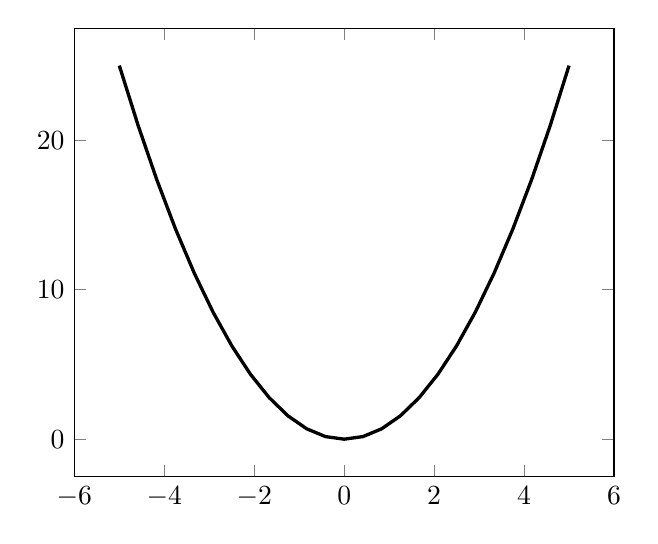
\begin{tikzpicture}
\begin{axis}[]
\addplot [black, very thick]{x*x};
\end{axis}
\end{tikzpicture}

\chapter{Praktiskā daļa}
\section {Darbs ar GEDA programmām}
\subsection{darbs ar gschem}

\begin{figure}[h]
\rotatebox{-90}{{\includegraphics[width=10cm,trim={3cm 3cm 3cm 3cm}]{01.ps}}}
\caption{GSCHEM elektriskā shēma}
\label{2}
\end{figure}

\subsection{darbs ar gnetlist}
\verbatiminput{01.net}
\subsection{darbs ar ngspice}
\begin{figure}[h]
\includegraphics[width=7cm]{011.ps}
\includegraphics[width=7cm]{022.ps}
\caption{Gschem shēmas signālu grafiki }
\label{3}
\end{figure}


\section{Darbs ar QUCS}

\begin{figure}[]
\rotatebox{-90}{{\includegraphics[width=6cm,trim={1,3cm 1cm 16cm 21cm}]{atkaribu_grafiki.ps}}}
\caption{QUCS simulācijas shēma ar sweep parametriem }
\label{4}
\end{figure}

\begin{figure}[]
\rotatebox{-90}{{\includegraphics[width=7cm,trim={0cm 2,1cm 15,9cm 17cm}]{shema2.ps}}}
\caption{QUCS grafiks ar shēmas datiem }
\label{5}
\end{figure}

Izmantojot programu QUCS\cite{gramata1} tika izveidota shēma ar avotu un divām pretestībām.
Principiālā shēma-(Shēmas elementiem\cite{gramata2} tika piešķirti pirms tam izrēķināti nomināli un nosimulēta shēma.Shēmas izveide bija viegla un noderīga priekšmetos kā ETP.)
Līdzstrāvas simulācijas-(Tika izveidota Sweep simulācija,kurā bija attēloti simulācijas dati.Dati,kas tika atspoguļoti ir noderīgi,lai bez iedziļināšanās varētu noskaidrot shēmas datus.)
SWEEP simulācijas un grafiki-(Izmantojot grafika un tabulas funkciajs tika izveidots grafiks un tabula, kuras atspoguļo datus un sakarības par izveidoto shēmu.No šiem datiem var secināt daudzas svarīgas lietas par shēmu piemēram spriegumus un pretestības)



\begin{thebibliography}{9}
\bibitem{gramata1}
Textbook by Paul Horowitz and Winfield Hill
The Art of Electronics , Cambridge University Press , 1980.

\bibitem{gramata2}
Textbook by Adel Sedra and Kenneth C. Smith
Microelectronic circuits , 1982.
\end{thebibliography}
\end{document}
